\section{Attempts to construct a counterexample}\label{sec:search}

The search starts from an adversarial question: can a known periodic
free-fall orbit be adjusted until it lies exactly on the Pythagorean
curve? This is more directed than waiting for a long trajectory to nearly
return. It also tests whether the apparent scarcity of second brakes is
merely an artifact of sampling.

\subsection{Impose the geometric constraints in stages}

Normalize $m_3=r_{12}=1$. In the larger family where each mass equals its
opposite side, a valid nondegenerate triangle has
\begin{equation}\label{eq:general-tied}
 q_1=(-1/2,0),\quad q_2=(1/2,0),\quad
 q_3=(x,y),\quad
 x={m_2^2-m_1^2\over2},\quad
 y=\sqrt{m_2^2-(x+1/2)^2}>0.
\end{equation}
There are now two adjustable mass ratios. Periodic candidates in this
larger family need not be right triangles. Their remaining defect is
\begin{equation}\label{eq:defect}
 D=m_1^2+m_2^2-1.
\end{equation}
An exact zero of $D$ is required even to challenge the stronger conjecture
for real parameters. An integer counterexample additionally needs rational
$u=m_2/(1+m_1)$.

Our September 2026 campaign starts from six entries of Li and Liao's
unequal-mass catalogue~\cite{LiLiao}. In the numerical construction we solve
three independent second-brake equations together with two mass--side
matching equations, varying the two initial-position coordinates, two
mass ratios, and a regularized flight time. Levi--Civita coordinates
replace the selected pair separation by a complex square and slow the
clock near close approaches. An atlas of pair choices avoids relying on
one coordinate chart for every encounter. Analytic variational equations
supply the shooting derivatives; pseudo-arclength continuation recovers
seeds for which direct correction stalls.

\begin{table}[tb]
\centering
\small
\begin{tabular}{lrrrr}
\toprule
Seed & $m_1$ & $m_2$ & Second-brake time & $D$\\
\midrule
$F_1$ & .536940689 & .839991651 & 1.337970014 & $-.006108723$\\
$F_2$ & .485763526 & .878297063 & 1.413330015 & $+.007371934$\\
$F_3$ & .343754597 & .887462426 & 1.074865097 & $-.094243220$\\
$F_4$ & .335421060 & .903827720 & 1.133475174 & $-.070588165$\\
$F_5$ & .474742622 & .896107795 & 1.544076262 & $+.028389737$\\
$F_{30}$ & .594811647 & .801774973 & 6.289233824 & $-.003355997$\\
\bottomrule
\end{tabular}
\caption{Ordinary numerical periodic candidates in the larger
mass--opposite-side family. None is Pythagorean. Digits are displayed for
reproducibility, not as interval-certified enclosures. The flight time is
physical normalized time; twice this value would be a period at an exact
collision-free second brake. Seed names refer to catalogue origins, not
to established connected branches of solutions.}
\label{tab:candidates}
\end{table}

\begin{figure}[tb]
\centering
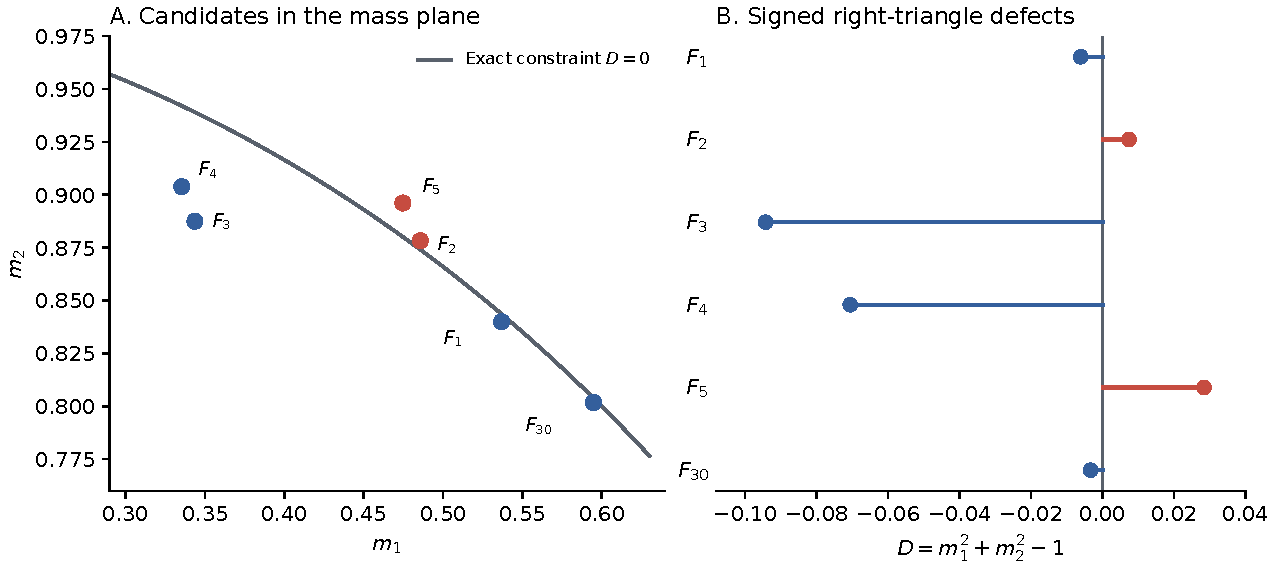
\includegraphics[width=.9\linewidth]{figures/counterexample-defects.pdf}
\caption{The six numerical candidates of Table~\ref{tab:candidates} and
exact right-triangle constraint. The left panel places them relative to
$m_1^2+m_2^2=1$; the right displays each signed defect directly. Opposite
signs at unrelated candidates are not an intermediate-value bracket.
No connecting solution branch is established by these points.}
\label{fig:defects}
\end{figure}

\subsection{What the numerical checks establish}

The corrected shooting residuals are at most about $1.2\times10^{-12}$.
Reintegration with an implicit Radau method, comparison with DOP853, and
backward reversal reproduce the candidate states to roughly
$2\times10^{-12}$. The corresponding five-equation Jacobians have
ordinary smallest singular values between approximately $0.199$ and
$0.870$ in the recorded physical-parameter convention. Their numerical
nonsingularity suggests isolated solutions of the five matching equations,
rather than freely adjustable families that automatically cross $D=0$.
It does not prove existence or isolation: those conclusions require a
validated implicit-function calculation.

The closest sampled separations range from about $3.4\times10^{-6}$ to
$5.0\times10^{-4}$. These values explain the use of regularization and
also limit the evidence: sampling alone does not certify positive
separation for every intervening time. Reconstructed energy is especially
sensitive to cancellation near the deepest passages; the campaign's worst
sampled physical energy error is about $2.5\times10^{-7}$. Small shooting
residuals must not be presented as equally small error bounds for every
physical observable.

We separately impose the exact right-triangle parameterization and look
for small kinetic energy at local maxima of the moment of inertia. Four
local searches seeded from $F_1,F_2,F_3,F_5$ converge to positive minima,
the smallest about $1.28\times10^{-4}$. The $F_{30}$ search reaches its
evaluation limit and remains noise-limited; the $F_4$ event correction
leaves the required strict-maximum branch. Neither incomplete search is
an exclusion theorem. No exact right-triangle second brake was found, so
there is no candidate on which rational reconstruction would be warranted.
Machine-readable results and exact replay commands accompany the campaign
report listed in Appendix~\ref{sec:reproduction}.

\subsection{Two tempting continuation arguments that do not suffice}

The defects of $F_1$ and $F_2$ have opposite signs. This would be useful if
we had a connected collision-free periodic branch joining them, on which
$D$ varied continuously. We do not. Their labelled half-orbit syzygy
sequences are different, and at zero angular momentum a noncollinear
collision-free orbit crosses every syzygy transversely. Consequently those
finite sequences cannot change on a connected finite-flight-time brake
family without an excluded event or endpoint. Opposite defects alone are
not a bracket.

Nor does a rank deficiency automatically construct the missing branch.
For five smooth equations in five unknowns, a rank-four Jacobian leaves
one direction to inspect, but the remaining scalar equation after
Lyapunov--Schmidt reduction can be $s^2=0$, with an isolated root. A branch
requires that residual equation to vanish along the proposed continuation.
Similarly, raw free-group words from the catalogue do not distinguish
these brake loops: a full brake orbit retraces its path and its loop in
collision-free shape space is null-homotopic. The ordered, labelled
syzygy sequence is the useful finite-itinerary information here.

The search has therefore produced well-tested near misses and sharper
requirements for a counterexample. It has not supplied a probability of
nonexistence, a numerical proof of the conjecture, or an obstruction to
unsearched long-period families.
